Before starting the development of the project, research shown that a few prototypes are currently in development with similar specifications. These projects present a variety of functionalities but due to the simplicity of the systems, all of them are addressed to educational field.

However, all of them present some different strengths and weaknesses. For instance, Pi-Bot \cite{PiBot} project runs using an Arduino prototyping board, fact that does not allow camera features unless the system is upgraded to a Raspberry Pi board. 

Furthermore, there are two remarkable projects currently on the field. Both of them are based on Raspberry Pi using PiCamera and wireless connection: GoPiGo \cite{GoPiGo} and TiddlyBot \cite{TiddlyBot}. 

On one hand, GoPiGo project is a complete kit that turns the Pi into a fully operating robot open for developers. However, it does not provide any functionality more than the hardware itself.

On the other hand, TiddlyBot it is a little bit more complete. For instance, the software package provides some amazing features such as draws, follow lines, and helps with the learning of technology. Additionally, it s possible to drive round your house using a tablet, smartphone or computer streaming the Pi's camera back to your device.

\begin{figure}
     \centering
     \begin{subfigure}[b]{0.3\textwidth}
             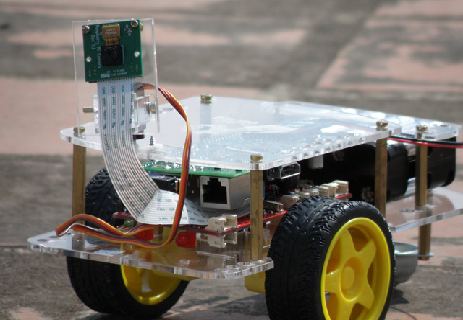
\includegraphics[width=\textwidth]{GoPiGo.png}
             \caption{GoPiGo}
             \label{fig:GoPiGo}
     \end{subfigure}%
     ~
     \begin{subfigure}[b]{0.3\textwidth}
             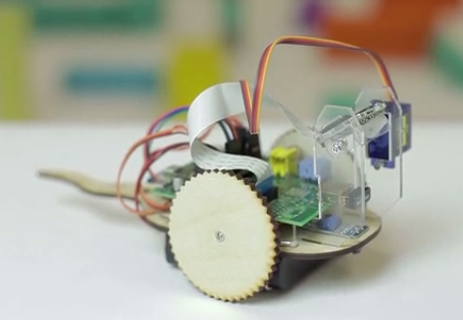
\includegraphics[width=\textwidth]{TiddlyBot.png}
             \caption{TiddlyBot}
             \label{fig:TiddlyBot}
     \end{subfigure}
     \caption{Similar educational robots}\label{fig:robots}
\end{figure}